\documentclass[twoside,11pt]{article}
\usepackage{pgm}



\usepackage[english]{babel}
\usepackage{hhline}
\usepackage[table]{xcolor}
\usepackage{pgf, tikz}
\usetikzlibrary{arrows, automata}
\usepackage{float}
\restylefloat{table}
\usepackage{tabularx,ragged2e,booktabs,caption}
\usepackage{makecell}
\usepackage{float}
\usepackage{amsmath}
\usepackage{latexsym}
\usepackage{amsfonts}
\usepackage{amssymb}
\usepackage{multirow}
\usepackage{pdflscape}
\usepackage{relsize}
\usepackage{url}
\usepackage{graphicx}
\usepackage{subcaption}
\usepackage{bm}
\usepackage{enumitem}
\usepackage{graphicx}
\usepackage[titlenotnumbered,algoruled,longend]{algorithm2e}
\usepackage{colortbl}

\usepackage[utf8]{inputenc}
\inputencoding{utf8}

\usepackage{hyperref,color,soul,booktabs}
\setulcolor{blue}
\newcommand{\BibTeX}{\textsc{B\kern-0.1emi\kern-0.017emb}\kern-0.15em\TeX}


\ShortHeadings{Bayesian Network Structure Learning with Side Constraints}{Li and van Beek}

\title{ Bayesian Network Structure Learning with Side Constraints }

\author{\Name{Andrew C. Li} \Email{acli@uwaterloo.ca}\and
   \Name{Peter van Beek} \Email{vanbeek@cs.uwaterloo.ca}\\
   \addr 	David R. Cheriton School of Computer Science  \\
	University of Waterloo \\ }

\begin{document}
\maketitle

% Abstract and keywords
\begin{abstract}%   <- trailing '%' for backward compatibility of .sty file
The abstract is a mandatory element that should summarize the contents of the paper. It should be confined within a single paragraph.
\end{abstract}
\begin{keywords}
We would like to encourage you to list your keywords here. They should be separated by semicolons and the last is followed by a full stop.
\end{keywords}

%
% Provide a clear statement of the problem addressed in the paper.
%
% Provide motivation for the problem.
% Why is the problem interesting? important? challenging?
%
% Review of previous work. Describe the work that other researchers
% have done on this problem and show why these previous approaches
% are inadequate (or put this in a separate section or subsection).
%
% Provide a summary of results.
%
\section{Introduction}

A Bayesian network (BN) is a probabilistic graphical model of a probability distribution
with applications in various fields, e.g. medicine \citep{Flores2011}, ecology \citep{Pollino2007},
and bioinformatics \citep{Friedman2000}. 

\medskip
In practice, BNs are usually either fully specified by an expert or learned directly from observed data, however,
both approaches have major drawbacks. Experts usually do not have enough domain knowledge to produce the
full network, especially as the number of random variables increases. On the other hand, the task of learning the 
BN structure directly from data is NP-hard, even to approximate to within a reasonable factor 
\citep{ChickeringMH03,Dasgupta1999} and data is often limited or expensive.

\subsection{Expert Knowledge Constraints.}
In many fields, hybrid methods for BN structure learning that incorporate both expert knowledge and data
have been applied to obtain superior results (see, e.g. \cite{Flores2011, Sesen2013, Oyen2016, Antal2004}).
We focus on \emph{score-and-search} based BN structure learning, incorporating prior knowledge as \emph{hard
constraints}; i.e. finding the optimal directed acyclic graph (DAG) that satisfies all constraints. Our method builds on MINOBS, a local search based
memetic algorithm for BN structure learning by \cite{Lee2017}. We are able to handle the following types of constraints in our
method.

\begin{enumerate}[label=({\arabic*})]
	\item \emph{Existence of an arc:} assert that a directed arc $xy$ exists. The user can also specify that an undirected arc $xy$ exists if the direction is not known.
	
	\item \emph{Absence of an arc:} assert that the directed arc $xy$ does \emph{not} exist. 
	
	\item \emph{Ordering constraint:} assert $x$ comes before $y$ in some topological ordering of the nodes in the BN. This implies that there exists no directed $y, x$-path (but the converse does not necessarily hold).
	
	\item \emph{(Positive) Ancestral relation:} assert the existence of a directed $x, y$-path. 

\end{enumerate}

These constraints are expressive enough to indirectly handle some other common constraints, such as undirected arc absence (no arc $xy$ or $yx$),
causal tiers (grouping variables into tiers and only permitting arcs from a lower tier to a higher tier) and specifying root nodes and leaves.

\medskip

The primary challenge of our work was incorporating ancestral relation constraints. Unlike the other constraints, ancestral constraints
are considered neither \emph{structure-modular} nor \emph{order-modular} and are notoriously difficult to incorporate into the
structure learning process \citep{Chen2016}. However, ancestral constraints are important for a number of reasons. First, although ancestral
constraints are weaker than directed arc existence constraints, direct dependencies can only be known given a high degree of 
domain knowledge. Experts are more likely to provide useful information when less specific constraints can also be asserted \citep{Flores2011}.
Secondly, ancestral constraints can be used to assert that one variable is an indirect cause of another, which is an abundant form of expert
knowledge in many domains (e.g. \cite{Sahin2006, Ma2017, Leu2013, Chen2014, Giordano2013}). Thirdly, BNs built for Bayesian inference
or prediction should encode all causal dependencies known to be correct. In our experimental evaluation, we demonstrate that imposing ancestral
constraints produces a BN much closer to the ground truth network in terms of their causal statements. Another important note is that BN structure
learning from data alone cannot distinguish between causal relationships and correlation. For example, Figure 1a. shows the well known \emph{asia}
network and Figure 1b. shows a network that is indistinguishable by data from \emph{asia} as the two networks encode the same conditional dependencies.

\begin{figure}[t]
	\centering
	\begin{subfigure}[t]{0.45\textwidth}
		\centering
		\includegraphics[width=\textwidth]{asia1}
		\caption{\emph{asia} network}
	\end{subfigure}
	\qquad
	\begin{subfigure}[t]{0.45\textwidth}
		\centering
		\includegraphics[width=\textwidth]{asia2}
		\caption{an I-equivalent network to \emph{asia}}
	\end{subfigure}
	\caption{}
\end{figure}

\subsection{Results.} We present a novel hybrid BN structure learning method that can incorporate expert knowledge as hard constraints,
including ancestral constraints. In our experimental evaluation, we demonstrate that our method is able to find high-quality solutions to 
constrained problems, while scaling to more variables than other existing methods. To the best of our knowledge, we are the first to 
successfully incorporate ancestral constraints into a local search based BN structure learning approach. 

\medskip
In Appendix A, we also describe some novel methods for handling other \emph{non-structure-modular} and \emph{non-order-modular} 
constraints in local search using dynamic programming. 

%We also believe the hill climbing method we used to incorporate ancestral constraints can 
%potentially be applied in the future to other global constraints that are currently out of reach for local search algorithms. 
%One example is \emph{d-separation}, which allows an expert to assert conditional independence statements. 

\subsection{Related work.} In recent years, researchers have devoted significant effort towards incorporating expert knowledge into
BN structure learning algorithms. We briefly discuss some of the most relevant work.

\medskip
\cite{CamposC07} produced a local search method  handling precisely the constraints (1) - (3). It is
worth mentioning that their local search method is based on the space of DAGs while our proposed method primarily searches
over the space of topological orderings. As constraints (1) - (3) are all \emph{structure-modular} or \emph{order-modular}, our
method can handle these in a straightforward way while additionally reducing the search space. Unfortunately this is not true of ancestral
constraints, which increase the running time when imposed.

\medskip
A recent approach by \cite{Chen2016} called EC Tree was specifically built to handle ancestral constraints. Note
that EC Tree can also handle constraints asserting the absence of a directed path and finds solutions with guaranteed optimality
which our proposed method cannot. They reported handling instances up to $n = 20$ random variables using the BDeu score.

\medskip
Another exact approach is the widely-used GOBNILP \footnote{www.cs.york.ac.uk/aig/sw/gobnilp/} which is able to handle a large variety of
constraints. Most notably, they are the only solver (to the best of our knowledge) capable of handling arbitrary conditional independence
constraints. Chen at. al. demonstrated that GOBNILP can be made to handle ancestral constraints, but requires orders of magnitude
more time than EC Tree.

\medskip
Causal discovery via MML (CaMML) \footnote{http://bayesian-intelligence.com/software/} is a stochastic search solver based on Markov Chain Monte Carlo
that is widely used in application fields. It is capable of handling all of the constraints (1)-(4) except for (2) i.e. arc absence. One is also able to
assert that two variables are correlated (i.e. not independent) and all constraints can be specified as a soft constraint by setting confidence levels. We will 
compare CaMML with our proposed method in our experimental evaluation. 


%
% Background material. Include enough background material so that
% the paper will be understandable to the intended audience.
%
\section{Background}
\label{SECTION:Background}

We begin by reviewing preliminary details on Bayesian networks (BNs) and the \emph{Bayesian network structure learning problem}. 

\medskip

A BN consists of a DAG $G$ with nodes $V = \{v_1, \ldots , v_n\}$, where each node is a random variable, and a conditional probability distribution
$P(v_i \text{ }| \text{ par}(v_i))$ for each random variable $v_i$, where $\text{par}(v_i)$ is the set of parents of $v_i$ in $G$. Arcs in $G$ from one node to another
represent direct dependencies, and the full structure $G$ encodes all conditional dependencies between the $n$ variables. 

\medskip

In this paper, we will focus on the \emph{score-and-search} method for BN structure learning. A scoring function $\sigma( \mathit{G} \mid D )$ is chosen where
every DAG $G$ on $n$ variables is assigned a score based on how well $G$ fits the data $D$ (we will assume a lower score is better). For convenience, we may simplify 
the notation to $\sigma( \mathit{G} )$, omitting $D$ which is assumed to be a constant set of data points. 

\medskip
A penalty term based on the complexity of $G$ is commonly used to
avoid overfitting.

\medskip

\begin{definition}[\textbf{Bayesian network structure learning problem}]
Given a data set $D = \{d_1, \ldots, d_N\}$, where $d_i$
is a vector of discrete values over features/random variables
$\mathit{V}$, and a scoring function $\sigma$ that measures how
well a candidate structure is supported by the observed data,
the \emph{Bayesian network structure learning problem} is to
find a directed acyclic graph $\mathit{G}$ over $\mathit{V}$
that minimizes the score $\sigma( \mathit{G} \mid D )$.
\end{definition}


\bigskip

A common property of most scoring functions, such as MDL/BIC \citep{Schwarz78}, and BDeu \citep{HeckermanGC95}, is \emph{decomposability}, meaning the score of 
the DAG is the sum of its local scores at each node: 

$$\sigma( \mathit{G} ) = \sum_{i = 1}^{n} \sigma(v_i,\text{ par}(v_i))$$

It is common practice to precompute the scores for each random variable $v_i$ and each candidate parent set $p \subseteq 2^{V \setminus \{v_i\} }$. \emph{Parent set
identification} involves pruning parent sets that never appear in optimal scoring solutions, often significantly reducing the number of candidate parent sets considered. We will further 
discuss this in Section 3. \emph{Structure optimization} is the task of assigning a parent set for each node to achieve a minimum scoring network with no cycles.


\medskip

Finally, we review the ordering-based search \citep{TeyssierK05} approach to BN structure learning that is used by MINOBS. Given a topological ordering $\mathcal{O}$ of the nodes, the optimal DAG consistent with $\mathcal{O}$ can be found in polynomial time, assuming parent sets are restricted to some constant size at most $k$. Specifically, the parents of $v_i$ must occur before $v_i$ in $\mathcal{O}$, and the parent set for each variable can be chosen independently from one another. Finding the optimal DAG consistent with
 $\mathcal{O}$ takes $O(Cn)$ time, where $C \in O(n^k)$ is the total number of candidate parent sets. The \emph{ordering-based search} approach is to search over the 
 space of orderings of $n$ variables using local search techniques, where the score of an ordering is the minimum score of a BN consistent with that ordering. MINOBS performs
 hill climbing with respect to an \emph{insert neighbourhood}, by choosing a variable in the ordering and inserting it at another index. For example, if the current ordering in the search is
 $(X_1, X_2, X_3, X_4)$, then $(X_1, X_4, X_2, X_3)$ is an insert neighbour (by inserting $X_4$ to index 2) and is therefore a candidate for the next ordering in the search. 
 For more details on how ordering-based search is used in MINOBS, refer to \cite{Lee2017}.

\medskip 
In order to incorporate prior knowledge, we wish to solve the BN structure learning problem with additional hard constraints (i.e. types (1)-(4) in Section 1) specified by an expert. We formally present the problem we will focus on for this paper.

\begin{definition}[\textbf{Constrained Bayesian network structure learning problem}]

Given a data set $D = \{d_1, \ldots, d_N\}$, where $d_i$
is a vector of discrete values over features/random variables
$\mathit{V}$, a scoring function $\sigma$ that measures how
well a candidate structure is supported by the observed data,
and arbitrarily many constraints of one of the following forms:

\begin{enumerate}

\item $x \rightarrow y$ (directed arc existence) or  $x \text{ \textemdash \  } y$ (undirected arc existence)
\item $x \nrightarrow y$ (directed arc absence)
\item $x < y$ (topological ordering constraint)
\item $x \rightsquigarrow y$ (ancestral constraint)

\end{enumerate}

the \emph{constrained Bayesian network structure learning problem} is to
find a directed acyclic graph $\mathit{G}$ over $\mathit{V}$ minimizing the score $\sigma( \mathit{G} \mid D )$ subject to
the following:

\begin{itemize}

\item for every constraint $x \rightarrow y$, the arc $xy$ is in $G$.
\item for every constraint $x \text{ \textemdash \  } y$, one of the arcs $xy$ or $yx$ is in $G$.
\item for every constraint $x \nrightarrow y$, the arc $xy$ is \emph{not} in $G$
\item there exists an ordering $\mathcal{O}$ such that for all constraints $x < y$, $x$ comes before $y$ in $\mathcal{O}$ and $\mathcal{O}$ is a
	topological ordering for $G$
\item for every constraint $x \rightsquigarrow y$, there exists a directed path from $x$ to $y$ in $G$

\end{itemize}
\end{definition}


\medskip
The rest of the paper will describe the methods used to incorporate the above constraints. 


%
% Statement of technical solutions. Provides a clear statement of the
% techniques used to solve the problem. Shows how the problem was
% approached, by what methods and techniques.
%
\section{Parent Set Identification}
\label{SECTION:ParentSetIdentification}

The vast majority of score-and-search approaches to BN structure learning use effective pruning strategies to reduce the number of candidate parent sets for each
variable. The problem of \emph{parent set identification} is to determine which parent sets do not appear in optimal solutions and hence do not need to further be considered.
Unfortunately, the optimal solution is unlikely to be feasible when additional hard constraints are imposed, and standard pruning techniques may remove some or all feasible
solutions from the search space. 

\medskip
For example, consider the following widely used pruning rule.

\begin{lemma}[\cite{CamposJ11}]

Let $X_i$ be a node, $\Pi, \Pi'$ potential parent sets for $X_i$ such that 
$\Pi \subset \Pi'$ and $\sigma(X_i, \Pi) < \sigma(X_i, \Pi')$. Then $\Pi'$ is
not the parent set of $X_i$ in an optimal DAG $G^*$. 
\end{lemma}

In the \emph{(unconstrained) BN structure learning problem}, this rule allows $\Pi'$ to be pruned since for any DAG $G'$ containing $\Pi'$ as a parent of $X_i$, 
one can instead assign $\Pi$ as the parent of $X_i$ resulting in a DAG $G$ with a strictly lower score than $G'$. However, when the addition of constraints are considered, this rule 
no longer holds, as $G'$ may satisfy arc existence or ancestral constraints that $G$ does not. In other words, it is still possible for $G'$ to be the optimal solution
to the \emph{constrained BN structure learning problem}, and therefore this pruning technique should not be used. 

\medskip

Our method uses new approaches to parent set identification specific to our needs. In particular, notice that the constraints can provide useful information for pruning. 

\medskip
If $x \rightarrow y$, then:

	\begin{itemize}
	\item any parent set of $y$ that does not contain $x$ can be pruned. (P1)
	\end{itemize}
	
If $x \nrightarrow y$, then:
	\begin{itemize}
	\item we may prune all parent sets of $y$ containing $x$. (P2)
	\end{itemize}

If $x < y$, then:
	\begin{itemize}
	\item we may prune parent sets of $x$ containing $y$. (P3)
	\end{itemize}
	
If $x \rightsquigarrow y$, then:
	\begin{itemize}
	\item if $\Pi$ is a parent set of $y$, and for all nodes $p \in \Pi$, if $p < x$, then $\Pi$ may be pruned (since assigning $\Pi$ as the parent set of $y$ immediately makes
		satisfaction of $x \rightsquigarrow y$ impossible). (P4)
	\end{itemize}
	
\bigskip

If we use this set of rules to prune the candidate parent sets, notice that any DAG constructed from the remaining candidate parent sets must automatically satisfy 
all constraints of the form $x \rightarrow y$ and $x \nrightarrow y$. If we wish to only consider DAGs consistent with some ordering $\mathcal{O}$, 
we can easily handle the constraint $x \text{ \textemdash \  } y$ using (P1) as the direction of the arc can be deduced from $\mathcal{O}$. Note, however, that 
parent sets pruned by the constraint $x \text{ \textemdash \  } y$ may be valid again when a different ordering is considered so we can only temporarily prune these parent sets.
We also observe that the ordering constraint $x < y$ can be inferred given either $x \rightarrow y$ or $x \rightsquigarrow y$. Furthermore, given ordering constraints $x < y$ and $y < z$, one can infer $x < z$. In a preprocessing step, our method infers a maximal set of ordering constraints as these constraints are extremely useful for parent set pruning and reducing the search space of orderings (as explained in Section 5). 


\medskip

The aforementioned pruning rules (P1) - (P5) are all \emph{lossless}, i.e. they do not prune the optimal solution to the \emph{constrained BN structure learning problem}. 
As a matter of fact, all solutions pruned are infeasible with respect to the set of constraints. We employ another pruning technique that is not guaranteed to be lossless, but is 
effective in drastically reducing the number of candidate parent sets.

\bigskip
\emph{
Let $X_i$ be a node, $\Pi, \Pi'$ potential parent sets for $X_i$, $\lambda \ge 1$ a constant such that 
$\Pi \subset \Pi'$ and $\lambda \sigma(X_i, \Pi) <  \sigma(X_i, \Pi')$. Then $\Pi'$ is
pruned from the set of candidate parent sets.
}
\begin{flushright}
(P6)
\end{flushright}

\bigskip
Notice that this pruning rule is equivalent to the pruning rule in Lemma 1 if $\lambda = 1$ is chosen. In general, this rule prunes a subset of the parent sets that
otherwise would have been pruned by Lemma 1. We prune a parent set $\Pi'$ if its score is significantly worse than one of its subsets $\Pi$, as $\Pi'$ is unlikely to appear in
optimal solutions to the \emph{constrained BN structure learning problem}. The choice of $\lambda$ is important; pruning too much can be detrimental to the quality of DAGs found while pruning too little is inefficient. We compute an initial value of $\lambda$ using the following formula.

$$\lambda = 1 + \omega (\frac{n}{N})(1 - (1 - \frac{m_{\text{anc}}}{n(n-1)})^2)$$

(where $n$ is number of random variables, $N$ is number of data points, $m_{\text{anc}}$ is number of 
ancestral constraints, and $\omega$ is a constant)

\medskip
This formula satisfies several key desiderata. Consider $G$ and $H$, the optimal-scoring DAGs without and with ancestral constraints imposed, respectively. 
When the number of data points is sufficiently large, we expect both $G$ and $H$ to be close to the ground truth network (or some I-equivalent network) and
also close in score. Therefore, we wish to have a smaller value for $\lambda$ to prune parent sets with poor scores more liberally with rule (P6). Note that
$\frac{n}{N}$ is used to measure the amount of data with respect to the problem size.

\medskip
Also, we expect $G$ and $H$ to be closer in score when the number of ancestral constraints is small. $\frac{m}{n(n-1)}$ measures how constrained
the problem instance is (note that $n(n-1)$ is an upper bound on the number of ancestral constraints) and hence it is desirable for $\lambda$ to be small
when $\frac{m}{n(n-1)}$ is small. The factor $1 - (1-\frac{m}{n(n-1)})^2$ is similar in behaviour to $\frac{m}{n(n-1)}$ but we found the former to perform
better when the number of constraints is small. 

\medskip
In our approach, we included the ability to restart the program with a higher value of $\lambda$ if the current candidate parent sets do not seem to yield
feasible solutions. Specifically, we restart with a new value of $\lambda' = 1 + 2(\lambda - 1)$.

\medskip
We will describe how the constant $\omega$ is selected in the experimental evaluation.


% Hill Climbing for Constraint Satisfaction
\section{Constraint-based Hill Climbing}
\label{SECTION:ConstraintBasedHillClimbing}

\begin{algorithm}[t]
	\caption{hillClimbDAG($G$, $\mathcal{O}$)}
 		allParents $\leftarrow$ allParentSets() \tcc*[r]{sorted by increasing score} 
		
		\While {true} {
			\For {$p$ in allParents} {
				$x$ $\leftarrow$ child($p$) \;
				\If {not tabu$(x)$ and feasible$(p, \mathcal{O})$} {
					$G'$ $\leftarrow$ $G$\;
					$G'$.parentOf($x$) $\leftarrow$ $p$ \;
					\If {$G'$ improves $G$} {
						$G$ $\leftarrow$ $G'$ \;
						break \;
					}
				}
			}
			
			\If {no improvement found} {
				\eIf {random$(0,1)$ $<$ walkProb} { 
					$p$ $\leftarrow$ random feasible parent set\;
					$x$ $\leftarrow$ child($p$) \;
					$G$.parentOf($x$) $\leftarrow$ $p$ \;
					tabu $x$ for $3$ iterations \;
				}
				 {
					break \;
				}
			}
			
		}
	
	return $G$ \;
\end{algorithm}


\begin{algorithm}[t]
	\caption{bestDAGForOrdering($\mathcal{O}$)}
 		$G$ $\leftarrow$ initialDAG($\mathcal{O}$) \;
		return hillClimbDAG($G$, $\mathcal{O}$) \;
\end{algorithm}


In this section, we discuss how to search for an optimal solution consistent with a given ordering $\mathcal{O}$ that simultaneously satisfies all constraints. Recall from the previous
section that  $x \rightarrow y$ and $x \nrightarrow y$ are handled in the parent set identification stage and since we are provided $\mathcal{O}$, 
$x \text{ \textemdash \  } y$ can also be handled. We assume that $\mathcal{O}$ is consistent with all ordering constraints (including those implied
by other constraints) as this is handled in the ordering-based search, detailed in Section 5. Therefore, we only need to consider ancestral constraints, $x \rightsquigarrow y$.
For convenience, we denote $\phi($G$)$ to be the number of ancestral constraints $x \rightsquigarrow y$ that are satisfied by the DAG $G$.

\begin{definition} [Parent assignment neighbour]

We say that two DAGs $G$ and $G'$ with the same nodes
are \emph{parent assignment neighbours} if and only if the parent set of a single node differs between $G$ and $G'$.
\end{definition}

\medskip

Algorithm 1 and Algorithm 2 outline the hill climbing method used to find a DAG satisfying all ancestral constraints. An initial DAG $G$ is chosen by assigning
a minimum-scoring parent set $p_i$ to each node $v_i$ such that each parent in $p_i$ occurs before $v_i$ in $\mathcal{O}$. It so happens that $G$ is the minimum cost
DAG consistent with $\mathcal{O}$ but $G$ may not necessarily satisfy all ancestral constraints. We then perform hill climbing on $G$ as described in Algorithm 1.

\medskip
At each iteration of the hill climb, we choose an \emph{improving parent assignment neighbour} $G'$ of $G$, replacing $G$ with $G'$. 
Here, we say that $G'$ is an \emph{improvement} over $G$ if and only if $\phi(G') > \phi(G)$ or $\phi(G) = \phi(G'), \sigma(G') < \sigma(G)$. 
In other words, the hill climb is directed towards finding solutions satisfying the most ancestral constraints as a primary objective, 
with score optimization as a secondary objective. We iterate through the list of candidate parent sets, $\emph{allParents}$, which is sorted in increasing order of score. 
For each candidate parent set $p$ for node $v$, we consider $G'$, the \emph{parent assignment neighbour} of $G$ that results from assigning $p$ as the parent 
for $v$ in $G$. As the number of candidate parent sets can be quite large, we adopt a \emph{first improvement} neighbour selection strategy. 
We note that computing $\phi(G')$ can be quite expensive; in the worst case, we must perform a depth-first search for each ancestral constraint $x \rightsquigarrow y$,
checking if there exists an $x, y$-dipath. However, observe that a constraint $x \rightsquigarrow y$ that is satisfied in $G$
must be satisfied in $G'$ unless $v$ is a descendant of $x$ and an ancestor of $y$ in $G$. Furthermore, if a constraint $x \rightsquigarrow y$ is not satisfied in $G$,
then it is satisfied in $G'$ if and only if $v$ is an ancestor of $y$ and $v$ has a parent in $G'$ that was a descendant of $x$ in $G$. Thus, it is useful to precompute for $G$
 which ancestral constraints are satisfied, the descendants of nodes $x$ that appear on the left-hand side of an ancestral constraint, and the ancestors of 
nodes $y$ that appear on the right-hand side of an ancestral constraint. Furthermore, during the
computation of $\phi(G')$, we can keep track of an upper bound on the number of constraints that can be satisfied (i.e. by assuming all constraints not yet checked
will be satisfied). If this upper bound is at any point less than $\phi(G)$ we stop working on $G'$ as it cannot be an improvement over $G$. These methods are able to
significantly reduce the number of depth-first search computations when computing $\phi(G')$.


\medskip
Unfortunately, a problem with the \emph{parent assignment neighbourhood} is that it is small and the hill climbing algorithm can easily become stuck in low-quality 
local minima, making it difficult to find the optimal solution. We solve this by introducing random walks and a tabu list. When the hill climb reaches a local minimum, it moves 
to a random non-improving solution with some small probability \emph{walkProb}. The node whose parent set was affected is then declared tabu for the next 3 iterations of the hill climb
so the change is not immediately undone (while a node is tabu, it cannot have its parent set reassigned).

\section{Ordering-based Search}
\begin{algorithm}[t]
	\caption{exploreSwapAdjacentNeighbour($\mathcal{O}$, $G$, $i$)}
		$\mathcal{O}'$ $\leftarrow$ $(X_1, ..., X_{i+1}, X_i, ..., X_n)$ \;
		$G'$ $\leftarrow$ $G$ \tcc*[r]{Transform $G'$ into a valid DAG under $\mathcal{O}'$}
		
		\If {$G'$\emph{.parentOf}$(X_{i+1})$ contains $X_i$ } {
			$G'$.parentOf$(X_{i+1})$ $\leftarrow$ feasibleParent$(X_{i+1}, \mathcal{O'})$ \;
		}
		
		return hillClimbDAG$(G', \mathcal{O}')$ \;
\end{algorithm} 

In this section, we focus on hill climbing over the space of topological orderings. The score of an ordering $\mathcal{O}$ is the minimum value of $\sigma(G)$
for DAGs $G$ consistent with $\mathcal{O}$ and satisfying all constraints. As the true minimum-scoring DAG is difficult to find, we treat the best DAG found by
Algorithm 2 as the score for $\mathcal{O}$. Furthermore, any orderings that do not satisfy the ordering constraints can be ignored or equivalently
assigned a score of $\infty$. 

\medskip
We follow roughly the same search strategy and neighbourhood that is outlined in MINOBS 
\citep{Lee2017}. Specifically, MINOBS makes use of the \emph{insert neighbourhood} and \emph{swap-adjacent neighbourhood}. Simply, $\mathcal{O'}$ is an 
\emph{insert neighbour} of $\mathcal{O}$ if it results from selecting an element of $\mathcal{O}$ and inserting it to a new index (e.g. $\{A,B,C,D\}$ and $\{A,D,B,C\}$
are \emph{insert neighbours}). A \emph{swap-adjacent neighbour} of $\mathcal{O}$ is an ordering resulting from swapping an element of $\mathcal{O}$ with its preceding element 
(e.g. $\{A,B,C,D\}$ and $\{A,B,D,C\}$ are \emph{swap-adjacent neighbours}). Note that every \emph{swap-adjacent neighbour} of $\mathcal{O}$ is also an insert neighbour of $\mathcal{O}$. 

\medskip
In MINOBS, the following neighbour improvement selection strategy is used. A random pivot element $X_i$ is chosen from $\mathcal{O}$ and the \emph{insert neighbours}
of $\mathcal{O}$ as a result of re-inserting $X_i$ are considered. If an improvement is found, that improvement is immediately selected. Otherwise, a new pivot is chosen
and this process is repeated. A key observation is that the \emph{insert neighbours} of $\mathcal{O}$ caused by re-inserting $X_i$ can be traversed by a series of $n-1$ 
\emph{swap-adjacent} moves. For a \emph{swap-adjacent} neighbour $\mathcal{O'}$, its score can be calculated efficiently in the \emph{unconstrained BN structure learning 
problem} since it only affects the choice of parent sets for the two swapped elements. 

\medskip
Unfortunately, the score of a \emph{swap-adjacent} neighbour cannot be calculated as easily in the constrained version of the problem. However, we found the following
strategy to be effective. Let the current ordering be $\mathcal{O} = (X_1, ..., X_i, X_{i+1}, ..., X_n)$ and the best feasible DAG found consistent with $\mathcal{O}$ be $G$.
Suppose index $i$ is being swapped with index $i+1$. Then Algorithm 3 describes a method for finding a high-quality DAG consistent with 
$\mathcal{O}' = (X_1, ..., X_{i+1}, X_i, ... , X_n)$ (satisfying all constraints). We found that using $G$ as an initial starting point for hill-climbing on $\mathcal{O'}$
had significantly reduced the running time, as $G$ satisfies all ancestral constraints and is likely to be near a local minimum. A problem arises when the parent of 
$X_{i+1}$ in $G$ contains $X_i$, as $G$ is not feasible under $\mathcal{O'}$ but we resolve this by replacing the parent of $X_{i+1}$ with the lowest-scoring
feasible parent under $\mathcal{O'}$ (though $G$ may no longer satisfy all ancestral constraints).

\medskip
Lastly, we briefly describe a method for generating random (feasible) orderings as this is required by MINOBS. We begin by generating a random
permutation of the $n$ variables, $P$. We repeatedly select an ordering constraint $x < y$ (explicit or implied by other constraints) that is not satisfied
by $P$ and swap $x$ and $y$ in $P$. This is repeated until no ordering constraints are unsatisfied. 

%
% Evaluation of the proposal. Shows how successful our solutions were,
% and why they were successful. Provide convincing evidence in support
% of all claims. Carefully evaluate the strengths and limitations
% of the contribution. Some dimensions for evaluation include empirical
% results and theoretical analyses.
%
\section{Experimental Evaluation}
\label{SECTION:Experimental}

In our experiments, we compare our proposed method, denoted by MINOBSx, against the CaMML software. CaMML was chosen for comparison as it is widely
used in application fields (see, e.g. \cite{Flores2011}, \cite{Kennett2001}, \cite{Sesen2013}) and is also based on a stochastic search-and-score approach. 
Unfortunately, the source code for EC Tree was not made available.

\medskip
Our test instances consist of all small and medium networks in the Bayesian Network Repository\footnote{http://www.bnlearn.com/bnrepository/}, the largest of 
which is \emph{barley} (48 nodes). For each network, we randomly sampled 6 small datasets and 6 large datasets. We ran two sets of experiments: 
(i) only using ancestral constraints and (ii) using various constraints. For each set of experiments, we selected 4 fixed percentages and sampled 5 sets of constraints
at that percentage (except for $100\%$ ancestral constraints, where there is only a single constraint set). We sampled each type of constraint in the following way
for a fixed percentage $p\%$. 

\begin{itemize}
\item We choose $p\%$ of all directed arcs in the true network. For each arc $xy$ we report $x \rightarrow y$ with probability $\frac{1}{2}$, otherwise we report 
$x \text{ \textemdash \  } y$.

\item We choose $p\%$ of all pairs $(x, y)$ such that there is no directed arc $xy$ and report $x \nrightarrow y$. 

\item We choose $p\%$ of all pairs $(x, y)$ such that there is a directed $x, y$-path and report $x \rightsquigarrow y$.

\item We use topological sort to retrieve an arbitrary topological ordering $\mathcal{O}$ and report $p\%$ of the $n \choose 2$ possible ordering constraints $x < y$ for
$\mathcal{O}$. 

\end{itemize}

\subsection{Setup.}

All tests were run on a single core of an Intel ``Broadwell" E5-2683 v4 CPU @ 2.1 Ghz with a memory limit of 512 MB for small networks and 4 GB for medium networks. 

\medskip
The parent set scores for MINOBSx were generated using GOBNILP with a parent limit of 3 (due to limited disk space) and the running time for GOBNILP is included in 
the total time taken for MINOBSx in the results. MINOBSx was run for 50 generations for small networks and 10 generations for medium networks. The parameter
$\omega$ described in Section 3 was tuned to a value of $50$ using the \emph{cancer}, \emph{child}, and \emph{barley} instances. 

\medskip
For CaMML, the search factor (controlling how extensively CaMML searches) was set to its default value. We allowed CaMML more running time than MINOBSx as CaMML
is implemented in Java while MINOBSx is implemented in C++. We specified all constraints with a confidence level of $1.0$ (indicating a hard constraint) except for ancestral
constraints, which were assigned a confidence of $0.9999$. We observed that CaMML was generally unable to find any solutions except on very small networks when the 
ancestral constraints were specified as hard constraints. Surprisingly, by changing the confidence to $0.9999$ for ancestral constraints, CaMML was able to completely solve
some instances that it otherwise was not able to find any solutions to. 

\subsection{Results.}

\begin{table}[H]
\captionof{table}{Results for small networks, with ancestral constraints only (first number in each pair) and with various constraints (second number in each pair).
$N$ is number of observations, $\%$ is the fixed percentage used to sample constraints, $\%$ feasible is the percentage of cases where the solution satisfied \emph{all} constraints imposed, $\%$ sat is the percentage of satisfied constraints out of those constraints imposed, $t$ is the running time required by the program. Highlighted cells indicate that not all
constraints were able to be satisfied.} 
\scriptsize
\renewcommand\theadfont{}
\centering
\begin{tabular}{  c | c | c || c | c | c || c | c | c }


\multirow{2}{*}{instance} & \multirow{2}{*}{$N$} & \multirow{2}{*}{$\%$} & \multicolumn{3}{c||}{MINOBSx} & \multicolumn{3}{c}{CaMML} \\ [2ex]
	& & &  \% feasible & \% sat & t  & \% feasible & \% sat & t  \\
	
\hhline {=|=|=||=|=|=||=|=|=}


%CANCER
\multirow{8}{*}{\thead{\textbf{cancer} \\ \\ 5 variables \\ 10 parameters}} & \multirow{4}{*}{250} & 10 / 5 & 100 / 100 & 100 / 100  & 0.1 / 0.1 & 100 / 100 & 100 / 100 & 4.0 / 3.9  \\

& & 25 / 10 & 100 / 100 & 100 / 100  & 0.1 / 0.0 & \cellcolor{yellow!100} 100 / 96.7 & \cellcolor{yellow!100} 100 / 98.9 & 4.1 / 4.0 \\
	
& & 50 / 15 & 100 / 100 & 100 / 100  & 0.1 / 0.1 & \cellcolor{yellow!100} 96.7 / 100 & \cellcolor{yellow!100} 99.2 / 100 & 4.2 / 4.3 \\

& & 100 / 20 & 100 / 100 & 100 / 100  & 0.1 / 0.0 &  100 / 100 & 100 / 100 & 4.2 / 4.2 \\

\hhline {~|-|-||-|-|-||-|-|-}

& \multirow{4}{*}{1000}

& 10 / 5 & 100 / 100 & 100 / 100 & 0.1 / 0.1 & \cellcolor{yellow!100} 96.7 / 100 & \cellcolor{yellow!100} 96.7 / 100 & 3.8 / 3.6 \\

& & 25 / 10  & 100 / 100 & 100 / 100  & 0.1 / 0.1 & 100 / 100 & 100 / 100 & 3.8 / 3.8 \\
	
& & 50 / 15 & 100 / 100 & 100 / 100 & 0.1 / 0.1 & 100 / 100 & 100 / 100 & 4.2 / 4.0 \\

& & 100 / 20 & 100 / 100 & 100 / 100 & 0.0 / 0.0 & 100 / 100 & 100 / 100 & 4.1 / 3.8 \\

\hhline {=|=|=||=|=|=||=|=|=}

%EARTHQUAKE
\multirow{8}{*}{\thead{\textbf{earthquake} \\ \\ 5 variables \\ 10 parameters}} & \multirow{4}{*}{250} 

& 10 / 5 & 100 / 100 & 100 / 100  & 0.1 / 0.1 & 100 / 100 & 100 / 100 & 4.2 / 4.3 \\

& & 25 / 10  & 100 / 100 & 100 / 100 & 0.1 / 0.1 & 100 / 100 & 100 / 100 & 4.3 / 4.5 \\
	
& & 50 / 15 & 100 / 100 & 100 / 100 & 0.1 / 0.0 & 100 / 100 & 100 / 100 & 4.4 / 4.1 \\

& & 100 / 20 & 100 / 100 & 100 / 100 & 0.1 / 0.0 & 100 / 100 & 100 / 100 & 4.5 / 4.1 \\

\hhline {~|-|-||-|-|-||-|-|-}

& \multirow{4}{*}{1000}

& 10 / 5 & 100 / 100 & 100 / 100 & 0.1 / 0.1 & 100 / 100 & 100 / 100 & 3.8 / 3.9 \\

& & 25 / 10  & 100 / 100 & 100 / 100 & 0.1 / 0.1 & 100 / 100 & 100 / 100 & 3.8 / 3.9 \\
	
& & 50 / 15 & 100 / 100 & 100 / 100 & 0.1 / 0.0 & 100 / 100 & 100 / 100 & 4.0 / 3.8 \\

& & 100 / 20 & 100 / 100 & 100 / 100 & 0.0 / 0.0 & 100 / 100 & 100 / 100 & 4.3 / 4.0 \\

\hhline {=|=|=||=|=|=||=|=|=}


%SURVEY
\multirow{8}{*}{\thead{\textbf{survey} \\ \\ 6 variables \\ 21 parameters}} & \multirow{4}{*}{250} 
& 10 / 5 & 100 / 100 & 100 / 100  & 0.2 / 0.1 & 100 / 100 & 100 / 100 & 4.7 / 4.6 \\

& & 25 / 10  & 100 / 100 & 100 / 100  & 0.3 / 0.1 & 100 / 100 & 100 / 100 & 5.0 / 4.6 \\
	
& & 50 / 15 & 100 / 100 & 100 / 100 & 0.2 / 0.1 & \cellcolor{yellow!100} 93.3 / 96.7 & \cellcolor{yellow!100} 99.0 / 99.4 & 4.9 / 4.4 \\

& & 100 / 20 & 100 / 100 & 100 / 100 &  0.1 / 0.1 & 100 / 100 & 100 / 100 & 4.9 / 4.4 \\

\hhline {~|-|-||-|-|-||-|-|-}

& \multirow{4}{*}{1000}

& 10 / 5 & 100 / 100 & 100 / 100 & 0.1 / 0.1 & \cellcolor{yellow!100} 96.7 / 96.7 & \cellcolor{yellow!100} 98.3 / 98.9 & 4.3 / 4.2 \\

& & 25 / 10  & 100 / 100 & 100 / 100 & 0.2 / 0.1 & \cellcolor{yellow!100} 96.7 / 96.7 & \cellcolor{yellow!100} 99.17 / 99.3 & 4.6 / 4.4 \\
	
& & 50 / 15 & 100 / 100 & 100 / 100 & 0.1 / 0.1 & \cellcolor{yellow!100} 93.3 / 93.3 & \cellcolor{yellow!100} 99.0 / 98.9 & 4.5 / 4.2 \\

& & 100 / 20 & 100 / 100 & 100 / 100 & 0.1 / 0.1 & \cellcolor{yellow!100} 100 / 96.7 & \cellcolor{yellow!100} 100 / 99.6 & 4.7 / 4.1 \\

\hhline {=|=|=||=|=|=||=|=|=}

%ASIA
\multirow{8}{*}{\thead{\textbf{asia} \\ \\ 8 variables \\ 18 parameters}} & \multirow{4}{*}{250} 

& 10 / 5  & 100 / 100 & 100 / 100 & 1.1 / 0.5 & 100 / 100 & 100 / 100 & 5.8 / 5.4 \\

& & 25 / 10 & 100 / 100 & 100 / 100 & 1.3 / 0.5  & 100 / 100 & 100 / 100 & 6.3 / 5.5 \\
	
& & 50 / 15 & 100 / 100 & 100 / 100 & 0.9 / 0.3 & 100 / 100 & 100 / 100 & 6.8 / 5.9 \\

& & 100 / 20 & 100 / 100 & 100 / 100  & 0.5 / 0.2 & 100 / 100 & 100 / 100 & 8.3 / 5.7 \\

\hhline {~|-|-||-|-|-||-|-|-}

& \multirow{4}{*}{1000}

& 10 / 5 & 100 / 100 & 100 / 100 & 0.9 / 0.4 & 100 / 100 & 100 / 100 & 5.5 / 5.0  \\

& & 25 / 10 & 100 / 100 & 100 / 100 & 1.1 / 0.4 & 100 / 100 & 100 / 100 & 6.0 / 5.3 \\
	
& & 50 / 15 & 100 / 100 & 100 / 100 & 0.7 / 0.3 & \cellcolor{yellow!100} 100 / 96.7 & \cellcolor{yellow!100} 100 / 99.7 & 6.3 / 5.6 \\

& & 100 / 20 & 100 / 100 & 100 / 100 & 0.4 / 0.2 & 100 / 100 & 100 / 100 & 7.3 / 5.6 \\

\hhline {=|=|=||=|=|=||=|=|=}


%SACHS
\multirow{8}{*}{\thead{\textbf{sachs} \\ \\ 11 variables \\ 178 parameters}} & \multirow{4}{*}{250} 

& 10 / 5  & 100 / 100 & 100 / 100 & 2.0 / 1.0 & 100 / 100 & 100 / 100 & 7.0 / 6.2 \\

& & 25 / 10 & 100 / 100 & 100 / 100 & 3.5 / 0.8 & \cellcolor{yellow!100} 100 / 93.3 & \cellcolor{yellow!100} 100 / 99.4 & 7.4 / 6.1  \\
	
& & 50 / 15 & 100 / 100 & 100 / 100 & 4.3 / 0.8 & 100 / 100 & 100 / 100 & 8.4 / 6.4  \\

& & 100 / 20 & 100 / 100 & 100 / 100 & 2.3 / 0.7 & \cellcolor{yellow!100} 16.7 / 100 & \cellcolor{yellow!100}  96.2 / 100 & 10.3 / 6.1 \\

\hhline {~|-|-||-|-|-||-|-|-}

& \multirow{4}{*}{1000}

& 10 / 5 & 100 / 100 & 100 / 100 & 1.6 / 1.0 & \cellcolor{yellow!100} 80.0 / 83.3 & \cellcolor{yellow!100} 93.3 / 97.2 & 6.2 / 5.9 \\

& & 25 / 10 & 100 / 100  & 100 / 100 & 2.5 / 0.8 & \cellcolor{yellow!100} 30.0 / 60.0 & \cellcolor{yellow!100} 87.8 / 94.8 & 7.2 / 6.0 \\
	
& & 50 / 15 & 100 / 100 & 100 / 100  &  2.9 / 0.6 & \cellcolor{yellow!100} 23.3 / 50.0 & \cellcolor{yellow!100} 90.0 / 96.9 & 8.1 / 6.2 \\

& & 100 / 20 & 100 / 100 & 100 / 100 & 2.2 / 0.6 & \cellcolor{yellow!100} 0 / 70.0 & \cellcolor{yellow!100} 95.5 / 98.5 & 9.9 / 6.3 \\


\end{tabular}
\end{table}

%%%%%%%%%%%%%%%%%%%%%%%%%%%%%%%%%%%%%%
\begin{table}[H]
\captionof{table}{Results for small networks, with ancestral constraints only (first number in each pair) and with various constraints (second number in each pair).
We report the number of missing, extra, and reversed arcs between the learned and true networks (the sum of these is the Hamming distance between DAGs),
the \emph{structural intervention distance} \citep{Peters2013} between the learned and true networks, which measures the difference in their respective causal statements (lower is better) and the percentage difference between the BDeu score and the baseline ($0^* \%$ row) BDeu score.}
\scriptsize
\centering
\renewcommand\theadfont{}
\begin{tabular}{ c | c | c || c | c | c | c | c  }
instance & $N$ &  \% & Missing & Extra & Reversed & SID &  Score (BDeu) \\

\hhline{=|=|=||=|=|=|=|=}

\multirow{10}{*}{\thead{\textbf{cancer} \\ \\ 5 variables \\ 10 parameters}}  & \multirow{5}{*}{250}

& $0^*$ & 1.8 & 0.2 & 0.8 & 9.2 & 0\% \\
& & 10 / 5 & 1.4 / 1.0 & 0.3 / 0.2 & 0.5 / 0.5 & 6.1 / 4.8 & 0.1\% / 0.1\% \\
& & 25 / 10 & 0.8 / 1.1 & 0.3 / 0.2 & 0.3 / 0.5 & 3.6 / 5.2 & 0.2\% / 0.2\% \\
& & 50 / 15 & 0.7 / 0.6 & 0.5 / 0.3 & 0.3 / 0.3 & 3.3 / 3.3 & 0.3\% / 0.3\% \\
& & 100 / 20 & 0.2 / 0.8 & 0.3 / 0.2 & 0.0 / 0.3 & 0.5 / 4.0 & 0.4\% / 0.2\% \\


\hhline{~|-|-||-|-|-|-|-}

& \multirow{5}{*}{1000}

& $0^*$ & 0.8 & 0.0 & 0.5 & 4.3 & 0\% \\
& & 10 / 5 & 0.7 / 0.6 & 0.1 / 0.0 & 0.5 / 0.4 & 4 / 3.1 & 0.0\% / 0.0\% \\
& & 25 / 10 & 0.5 / 0.5 & 0.2 / 0.1 & 0.3 / 0.5 & 2.6 / 3.4 & 0.1\% / 0.0\% \\
& & 50 / 15 & 0.3 / 0.3 & 0.1 / 0.1 & 0.1 / 0.1 & 1.0 / 1.4 & 0.1\% / 0.1\% \\
& & 100 / 20 & 0.0 / 0.4 & 0.0 / 0.0 & 0.0 / 0.3 & 0 / 2.3 & 0.1\% / 0.1\% \\

\hhline{=|=|=||=|=|=|=|=}

\multirow{10}{*}{\thead{\textbf{earthquake} \\ \\ 5 variables \\ 10 parameters}} & \multirow{5}{*}{250}

& $0^*$ & 0.8 & 1.0 & 1.5 & 8.7 & 0\% \\
& & 10 / 5 & 0.6 / 0.4 & 1.0 / 1.0 & 0.6 / 0.3 & 4.2 / 2.7 & 0.2\% / 0.3\% \\
& & 25 / 10 & 0.4 / 0.6 & 0.9 / 1.0 & 0.2 / 0.5 & 1.7 / 3.9 & 0.3\% / 0.3\% \\
& & 50 / 15 & 0.4 / 0.3 & 1.2 / 1.1 & 0.3 / 0.2 & 1.9 / 2.3 & 0.5\% / 0.7\% \\
& & 100 / 20 & 0.2 / 0.4 & 1.2 / 1.2 & 0.0 / 0.2 & 0.2 / 2.1 & 0.7\% / 0.6\% \\

\hhline{~|-|-||-|-|-|-|-} 
& \multirow{5}{*}{1000}

& $0^*$ & 0.0 & 0.5 & 0.3 & 1.5 & 0\% \\
& & 10 / 5 & 0.0 / 0.0 & 0.4 / 0.3 & 0.1 / 0.0 & 0.6 / 0 & 0.0\% / 0.0\% \\
& & 25 / 10 & 0.0 / 0.0 & 0.3 / 0.3 & 0.0 / 0.0 & 0 / 0.3 & 0.0\% / 0.0\% \\
& & 50 / 15 & 0.0 / 0.0 & 0.3 / 0.5 & 0.0 / 0.1 & 0 / 0.9 & 0.0\% / 0.1\% \\
& & 100 / 20 & 0.0 / 0.0 & 0.3 / 0.3 & 0.0 / 0.0 & 0 / 0 & 0.0\% / 0.1\% \\

\hhline{=|=|=||=|=|=|=|=}
\multirow{10}{*}{\thead{\textbf{survey} \\ \\ 6 variables \\ 21 parameters}} & \multirow{5}{*}{250} 

& $0^*$ & 4.5 & 0.0 & 0.5 & 15.5 & 0\% \\
& & 10 / 5 & 3.6 / 3.1 & 0.8 / 0.4 & 0.6 / 0.6 & 13.1 / 12.2 & 0.4\% / 0.4\% \\
& & 25 / 10 & 2.8 / 2.8 & 1.4 / 0.2 & 0.5 / 0.1 & 11.7 / 8.9 & 0.7\% / 0.5\% \\
& & 50 / 15 & 2.4 / 2.8 & 1.5 / 0.6 & 0.5 / 0.1 & 9.1 / 9.7 & 1.0\% / 0.7\% \\
& & 100 / 20 & 2.5 / 2.1 & 2.0 / 0.7 & 0.0 / 0.3 & 6.2 / 8.0 & 1.2\% / 1.0\% \\

\hhline{~|-|-||-|-|-|-|-} 
& \multirow{5}{*}{1000}
& $0^*$ & 3.5 & 0.0 & 1.3 & 16.3 & 0\% \\
& & 10 / 5 & 2.8 / 2.3 & 1.0 / 0.4 & 1.3 / 1.1 & 15.9 / 13.5 & 0.1\% / 0.1\% \\
& & 25 / 10 & 2.7 / 2.5 & 1.1 / 0.3 & 0.3 / 0.3 & 10.1 / 8.3 & 0.1\% / 0.1\% \\
& & 50 / 15 & 2.6 / 2.5 & 1.4 / 0.6 & 0.2 / 0.2 & 8.2 / 8.7 & 0.2\% / 0.2\% \\
& & 100 / 20 & 2.7 / 1.7 & 1.8 / 0.5 & 0.0 / 0.4 & 6.8 / 8.5 & 0.2\% / 0.3\% \\

\hhline{=|=|=||=|=|=|=|=}
\multirow{10}{*}{\thead{\textbf{asia} \\ \\ 8 variables \\ 18 parameters}} & \multirow{5}{*}{250} 
& $0^*$ & 1.5 & 1.7 & 1.0 & 12.2 & 0\% \\
& & 10 / 5 & 1.4 / 1.4 & 1.6 / 1.6 & 0.7 / 0.9 & 10.3 / 11.1 & 0.0\% / 0.0\% \\
& & 25 / 10 & 1.2 / 1.4 & 1.8 / 1.6 & 0.5 / 0.6 & 7.2 / 8.9 & 0.1\% / 0.1\% \\
& & 50 / 15 & 1.0 / 0.8 & 2.0 / 1.4 & 0.3 / 0.4 & 4.3 / 4.4 & 0.2\% / 0.3\% \\
& & 100 / 20 & 0.5 / 0.7 & 1.7 / 1.1 & 0.0 / 0.2 & 1.8 / 3.9 & 0.3\% / 0.3\% \\

\hhline{~|-|-||-|-|-|-|-} 
& \multirow{5}{*}{1000}
& $0^*$ & 0.8 & 0.3 & 1 & 9.0 & 0\% \\
& & 10 / 5 & 0.7 / 0.8 & 0.4 / 0.4 & 0.9 / 1.1 & 7.3 / 9.0 & 0.0\% / 0.0\% \\
& & 25 / 10 & 0.4 / 0.5 & 0.5 / 0.3 & 0.4 / 0.8 & 4.2 / 6.4 & 0.0\% / 0.0\% \\
& & 50 / 15 & 0.2 / 0.3 & 0.4 / 0.4 & 0.0 / 0.5 & 0.4 / 3.6 & 0.0\% / 0.0\% \\
& & 100 / 20 & 0.0 / 0.2 & 0.3 / 0.3 & 0.0 / 0.4 & 0 / 3.1 & 0.0\% / 0.0\% \\

\hhline{=|=|=||=|=|=|=|=}
\multirow{10}{*}{\thead{\textbf{sachs} \\ \\ 11 variables \\ 178 parameters}} & \multirow{5}{*}{250} 
& $0^*$ & 6.5 & 1.0 & 5.3 & 48.0 & 0\% \\
& & 10 / 5 & 6.0 / 5.0 & 0.8 / 0.5 & 3.5 / 3.4 & 36.2 / 34.7 & 0.2\% / 0.4\% \\
& & 25 / 10 & 5.5 / 4.5 & 0.6 / 0.3 & 2.6 / 1.7 & 33.4 / 24.8 & 0.3\% / 0.6\% \\
& & 50 / 15 & 4.9 / 3.9 & 0.3 / 0.2 & 1.4 / 1.5 & 24.5 / 22.0 & 0.5\% / 0.9\% \\
& & 100 / 20 & 3.2 / 3.5 & 0.0 / 0.0 & 0.0 / 0.8 & 15 / 16.2 & 0.9\% / 0.8\% \\

\hhline{~|-|-||-|-|-|-|-} 
& \multirow{5}{*}{1000}
& $0^*$ & 1.5 & 0.0 & 6.0 & 30.5 & 0\% \\
& & 10 / 5 & 1.3 / 1.1 & 0.0 / 0.0 & 4.1 / 3.7 & 22.2 / 20.7 & 0.0\% / 0.0\% \\
& & 25 / 10 & 1.1 / 0.5 & 0.0 / 0.0 & 3.4 / 1.8 & 20.7 / 13.8 & 0.0\% / 0.1\% \\
& & 50 / 15 & 0.9 / 0.8 & 0.0 / 0.0 & 2.6 / 2.2 & 15.9 / 13.6 & 0.1\% / 0.1\% \\
& & 100 / 20 & 0.5 / 0.5 & 0.0 / 0.0 & 0.0 / 1.4 & 1.5 / 10.4 & 0.1\% / 0.1\% \\

\end{tabular}
\end{table}

%%%%%%%%%%%%%%%%%%%%%%%%%%%%%%%%%%%%%%%

\begin{table}[H]
\captionof{table}{Results for medium networks, with ancestral constraints only (first number in each pair) and with various constraints (second number in each pair).}
\centering
\scriptsize
\renewcommand\theadfont{}
\begin{tabular}{  c | c | c || c | c | c || c | c | c }


\multirow{2}{*}{instance} & \multirow{2}{*}{$N$} & \multirow{2}{*}{$\%$} & \multicolumn{3}{c||}{MINOBSx} & \multicolumn{3}{c}{CaMML} \\ [2ex]
	& & &  \% feasible & \% sat & t  & \% feasible & \% sat & t  \\
	
\hhline {=|=|=||=|=|=||=|=|=}

%CHILD
\multirow{8}{*}{\thead{\textbf{child} \\ \\ 20 variables \\ 230 parameters}} & \multirow{4}{*}{500} 

& 10 / 5  & 100 / 100 & 100 / 100 & 11.2 / 7.2 & 100 / 100 & 100 / 100 & 66.8 / 58.4 \\
& & 25 / 10 & 100 / 100 & 100 / 100 & 29.9 / 7.3 & 100 / 100 & 100 / 100 & 86.0 / 62.4  \\
& & 50 / 15 & 100 / 100 & 100 / 100 & 37.8 / 4.1 & 100 / 100 & 100 / 100 & 120.6 / 64.6  \\
& & 100 / 20 & 100 / 100 & 100 / 100 & 26.1 / 5.1 & \cellcolor{yellow!100} 66.7 / 100 & \cellcolor{yellow!100}  99.5 / 100 & 197.6 / 64.6 \\

\hhline {~|-|-||-|-|-||-|-|-}

& \multirow{4}{*}{2000}

& 10 / 5 & 100 / 100 & 100 / 100 & 9.4 / 6.7 & 100 / 100 &  100 / 100 & 61.0 / 55.1 \\
& & 25 / 10 & 100 / 100  & 100 / 100 & 19.1 / 6.0 & 100 / 100 & 100 / 100 & 83.7 / 59.7 \\
& & 50 / 15 & 100 / 100 & 100 / 100  & 25.7 / 3.0 & 100 / 100 & 100 / 100 & 115.6 / 60.6 \\
& & 100 / 20 & 100 / 100 & 100 / 100 & 20.4 / 3.2 & 100 / 100 & 100 / 100 & 180.2 / 60.1 \\
 
\hhline {=|=|=||=|=|=||=|=|=}


\multirow{8}{*}{\thead{\textbf{insurance} \\ \\ 27 variables \\ 984 parameters}} & \multirow{4}{*}{500}
& 10 / 5  & 100 / 100 & 100 / 100 & 180.5 / 104.9 & \cellcolor{yellow!100} 50.0 / 70.0 & \cellcolor{yellow!100} 95.9 / 99.0 & 439.5 / 325.3  \\
& & 25 / 10 & 100 / 100 & 100 / 100 & 318.9 / 56.5 &\cellcolor{yellow!100}  56.7 / 50.0 & \cellcolor{yellow!100} 98.0 / 98.9 & 723.9 / 385.0  \\
& & 50 / 15 & 100 / 100 & 100 / 100 & 328.7 / 52.8 & \cellcolor{yellow!100} 30.0 / 33.3 & \cellcolor{yellow!100} 98.5 / 98.1 & 1165.6 / 485.2  \\
& & 100 / 20 & 100 / 100 & 100 / 100 & 292.5 / 37.4 & \cellcolor{yellow!100} 0 / 53.3 & \cellcolor{yellow!100} 98.1 / 99.6 & 2052.3 / 571.7 \\

\hhline {~|-|-||-|-|-||-|-|-}

& \multirow{4}{*}{2000}
& 10 / 5 & 100 / 100 & 100 / 100 & 124.0 / 88.3 &  \cellcolor{yellow!100} 0 / 53.3 &  \cellcolor{yellow!100} 78.8 / 98.1 & 438.5 / 309.8  \\
& & 25 / 10 & 100 / 100  & 100 / 100 & 236.3 / 49.6 & \cellcolor{yellow!100}  16.7 / 23.3 &  \cellcolor{yellow!100} 92.4 / 96.8 & 748.6 / 393.2 \\
& & 50 / 15 & 100 / 100 & 100 / 100  & 251.5 / 48.2 &  \cellcolor{yellow!100} 3.3 / 10.0 &  \cellcolor{yellow!100} 94.4 / 96.6 & 1175.2 / 487.9  \\
& & 100 / 20 & 100 / 100 & 100 / 100 & 233.1 / 33.4 & \cellcolor{yellow!100}  0 / 10.0  &  \cellcolor{yellow!100} 95.6 / 98.8 & 1956.8 / 571.1 \\

\hhline{=|=|=||=|=|=|=|=|=}
\multirow{8}{*}{\thead{\textbf{water} \\ \\ 32 variables \\ 10083 parameters}} & \multirow{4}{*}{1000} 
& 10 / 5 & 100 / 100 & 100 / 100 & 436.5 / 236.0 & \cellcolor{yellow!100} 86.7 / 100 &\cellcolor{yellow!100}  99.3 / 100 & 2740.5 / 2138.4 \\
& & 25 / 10 & 100 / 100  & 100 / 100 & 987.1 / 265.2 & \cellcolor{yellow!100} 80.0 / 43.3 & \cellcolor{yellow!100} 99.5 / 99.0 & 4934.6 / 2782.8 \\
& & 50 / 15 & 100 / 100 & 100 / 100  & 1083.2 / 166.0 & \cellcolor{yellow!100} 46.7 / 30.0 & \cellcolor{yellow!100} 99.2 / 98.9 & 8499.3 / 3239.0  \\
& & 100 / 20 & 100 / 100 & 100 / 100 & 1015.1 / 87.9 & \cellcolor{yellow!100} 16.7 / 30.0 & \cellcolor{yellow!100} 99.3 / 99.1 & 15299.3 / 3967.5 \\

\hhline {~|-|-||-|-|-||-|-|-}

& \multirow{4}{*}{4000}
& 10 / 5 & 100 / 100 & 100 / 100 & 358.9 / 232.5 & \cellcolor{yellow!100} 30 / 63.3 & \cellcolor{yellow!100} 92.2 / 98.9 & 2912.2 / 2153.3  \\
& & 25 / 10 & 100 / 100  & 100 / 100 & 788.7 / 169.2 & \cellcolor{yellow!100} 10.0 / 10.0 & \cellcolor{yellow!100} 94.5 / 98.4 & 5081.3 / 2725.6 \\
& & 50 / 15 & 100 / 100 & 100 / 100  & 901.6 / 139.2  & \cellcolor{yellow!100} 6.7 / 3.3 & \cellcolor{yellow!100} 95.3 / 97.7 & 8325.3 / 3377.0  \\
& & 100 / 20 & 100 / 100 & 100 / 100 & 934.6 / 62.0 & \cellcolor{yellow!100} 0 / 0 & \cellcolor{yellow!100} 98.5 / 97.6 & 15341.1 / 4210.0 \\

\hhline{=|=|=||=|=|=|=|=|=}
\multirow{8}{*}{\thead{\textbf{mildew} \\ \\ 35 variables \\ 540150 parameters}} & \multirow{4}{*}{8000} 

& 10 / 5 & 100 / 100 & 100 / 100 & 193.8 / 754.7 & \cellcolor{yellow!100} 0 / 0 & \cellcolor{yellow!100} 26.9 / 75.6 & 2134.2 / 1442.0  \\
& & 25 / 10 & 100 / 100  & 100 / 100 & 632.1 / 334.2 & \cellcolor{yellow!100} 0 / 0 & \cellcolor{yellow!100} 29.4 / 86.5 & 3906.5 / 1835.7 \\
& & 50 / 15 & 100 / 100 & 100 / 100  & 943.3 / 321.0 & \cellcolor{yellow!100} 0 / 0 & \cellcolor{yellow!100} 40.3 / 88.2 & 7336.1 / 2215.0  \\
& & 100 / 20 & 100 / 100 & 100 / 100 & 1085.4 / 309.7 & \cellcolor{yellow!100} 0 / 0 & \cellcolor{yellow!100} 54.4 / 89.8 & 12649.3 / 2572.5 \\

\hhline {~|-|-||-|-|-||-|-|-}
& \multirow{4}{*}{32000}
& 10 / 5 & 100 / 100 & 100 / 100 & 181.6 / 353.0  & \cellcolor{yellow!100} 0 / 0 & \cellcolor{yellow!100} 19.4 / 77.8 & 2553.9 / 1664.6  \\
& & 25 / 10 & 100 / 100  & 100 / 100 & 471.6 / 266.2 & \cellcolor{yellow!100} 0 / 0 & \cellcolor{yellow!100} 19.4 / 87.7 & 4763.4 / 1983.3 \\
& & 50 / 15 & 100 / 100 & 100 / 100  & 702.2 / 210.2 & \cellcolor{yellow!100} 0 / 0 & \cellcolor{yellow!100} 24.0 / 88.0 & 8546.6 / 2462.6  \\
& & 100 / 20 & 100 / 100 & 100 / 100 & 761.0 / 264.8 & \cellcolor{yellow!100} 0 / 0 & \cellcolor{yellow!100} 28.2 / 92.3 & 17148.3 / 2400.38 \\

\hhline{=|=|=||=|=|=|=|=|=}
\multirow{8}{*}{\thead{\textbf{alarm} \\ \\ 37 variables \\ 509 parameters}} & \multirow{4}{*}{1000} 
& 10 / 5 & 100 / 100 & 100 / 100 & 954.0 / 160.9 & \cellcolor{yellow!100} 86.7 / 96.7 & \cellcolor{yellow!100} 99.4 / 99.9 & 2423.0 / 1736.6 \\
& & 25 / 10 & 100 / 100  & 100 / 100 & 1893.2 / 316.9 & \cellcolor{yellow!100} 76.7 / 90.0 & \cellcolor{yellow!100} 99.5 / 99.9 & 4070.2 / 2019.4 \\
& & 50 / 15 & 100 / 100 & 100 / 100  & 1627.7 / 185.1 & \cellcolor{yellow!100} 73.3 / 100 & \cellcolor{yellow!100} 99.5 / 100 & 6753.0 / 2263.7  \\
& & 100 / 20 & 100 / 100 & 100 / 100 & 1207.2 / 147.3 & \cellcolor{yellow!100} 83.3 / 100 & \cellcolor{yellow!100} 99.9 / 100 & 12377.2 / 2692.7 \\

\hhline {~|-|-||-|-|-||-|-|-}
& \multirow{4}{*}{4000}
& 10 / 5 & 100 / 100 & 100 / 100 & 602.3 / 115.3 & \cellcolor{yellow!100} 70.0 / 83.3 & \cellcolor{yellow!100} 97.2 / 99.7 & 2314.6 / 1705.3  \\
& & 25 / 10 & 100 / 100  & 100 / 100 & 1336.8 / 224.7 & \cellcolor{yellow!100} 86.7 / 86.7 & \cellcolor{yellow!100} 99.3 / 99.9 & 3807.8 / 1988.3 \\
& & 50 / 15 & 100 / 100 & 100 / 100  & 1438.2 / 133.3 & \cellcolor{yellow!100} 90.0 / 100 & \cellcolor{yellow!100} 99.8 / 100 & 6268.1 / 2163.7 \\
& & 100 / 20 & 100 / 100 & 100 / 100 & 1195.6 / 116.5 & \cellcolor{yellow!100} 50.0 / 80.0 & \cellcolor{yellow!100} 99.0 / 99.8 & 11169.0 / 2581.8 \\

\hhline{=|=|=||=|=|=|=|=|=}
\multirow{8}{*}{\thead{\textbf{barley} \\ \\ 48 variables \\ 114005 parameters}} & \multirow{4}{*}{2000} 
& 10 / 5 & 100 / 100 & 100 / 100 & 2321.4 / 5866.8 & \cellcolor{yellow!100} 0 / 0 & \cellcolor{yellow!100} 70.3 / 89.3 & 19824.8 / 11666.1  \\
& & 25 / 10 & 100 / 100  & 100 / 100 & 4228.9 / 2941.3 & \cellcolor{yellow!100} 0 / 0 & \cellcolor{yellow!100} 74.4 / 93.6  & 37034.3 / 14864.9 \\
& & 50 / 15 & 100 / 100 & 100 / 100  & 7163.0 / 3518.9 & \cellcolor{yellow!100} 0 / 0 & \cellcolor{yellow!100} 73.9 / 95.0 & 70433.0 / 20339.2  \\
& & 100 / 20 & 100 / 100 & 100 / 100 & 7246.6 / 1806.3 & \cellcolor{yellow!100} 0 / 0 & \cellcolor{yellow!100} 80.9 / 96.3 & 114036.7 / 22366.9 \\

\hhline {~|-|-||-|-|-||-|-|-}
& \multirow{4}{*}{8000}
& 10 / 5 & 100 / 100 & 100 / 100 & 4761.1 / 6032.7 & \cellcolor{yellow!100} 0 / 0 & \cellcolor{yellow!100} 44.0 / 82.8 & 18092.6 / 10759.6 \\
& & 25 / 10 & 100 / 100  & 100 / 100 & 4063.8 / 3620.0 & \cellcolor{yellow!100} 0 / 0 & \cellcolor{yellow!100} 52.5 / 91.8 & 35308.3 / 14477.5 \\
& & 50 / 15 & 100 / 100 & 100 / 100  & 5137.8 / 3022.8 & \cellcolor{yellow!100} 0 / 0 & \cellcolor{yellow!100} 54.0 / 95.1 & 64893.5 / 18142.0  \\
& & 100 / 20 & 100 / 100 & 100 / 100 & 5675.6 / 1638.8 & \cellcolor{yellow!100} 0 / 0 & \cellcolor{yellow!100} 53.4 / 95.1 & 111338.4 / 21184.4 \\

\end{tabular}
\end{table}


%%%%%%%%%%%%%%%%%%%%%%%%%%%%%%%%%%%%%%
\begin{table}[H]
\captionof{table}{Results for medium networks, with ancestral constraints only (first number in each pair) and with various constraints (second number in each pair).} 
\scriptsize
\centering
\renewcommand\theadfont{}
\begin{tabular}{ c | c | c || c | c | c | c | c  }

instance & $N$ & \% & Missing & Extra & Reversed & SID & Score (BDeu) \\

\hhline{=|=|=||=|=|=|=|=}

\multirow{10}{*}{\thead{\textbf{child} \\ \\ 20 variables \\ 230 parameters}}  & \multirow{5}{*}{500}

& $0^*$ & 5.3 & 1.0 & 3.0 & 115.7 & 0\% \\
& & 10 / 5 & 4.8 / 4.8 & 1.1 / 0.8 & 1.9 / 1.3 & 91.4 / 82.6 & 0.1\% / 0.2\% \\
& & 25 / 10 & 4.7 / 4.3 & 1.9 / 1.6 & 1.6 / 1.8 & 93.9 / 79.4 & 0.2\% / 0.3\% \\
& & 50 / 15 & 3.9 / 4.2 & 1.4 / 1.2 & 1.7 / 0.7 & 76.1 / 69.9 & 0.3\% / 0.4\% \\
& & 100 / 20 & 2.2 / 3.6 & 2.2 / 0.8 & 0.0 / 0.3 & 35.8 / 57.6 & 0.9\% / 0.4\% \\


\hhline{~|-|-||-|-|-|-|-}

& \multirow{5}{*}{2000}

& $0^*$ & 1.7 & 0.2 & 3.5 & 79.2 & 0\% \\
& & 10 / 5 & 1.5 / 1.3 & 0.2 / 0.2 & 0.5 / 0.1 & 26.0 / 20.8 & 0.0\% / 0.0\% \\
& & 25 / 10 & 0.7 / 1.0 & 0.3 / 0.3 & 0.3 / 0.5 & 12.1 / 18.0 & 0.0\% / 0.0\% \\
& & 50 / 15 & 0.7 / 1.0 & 0.3 / 0.3 & 0.5 / 0.0 & 12.2 / 16.2 & 0.0\% / 0.0\% \\
& & 100 / 20 & 0.2 / 1.0 & 0.3 / 0.1 & 0.0 / 0.0 & 2.5 / 16.6 & 0.1\% / 0.0\% \\

\hhline{=|=|=||=|=|=|=|=}

\multirow{10}{*}{\thead{\textbf{insurance} \\ \\ 27 variables \\ 984 parameters}} & \multirow{5}{*}{500}

& $0^*$ & 18.8 & 4.0 & 2.8 & 348.2 & 0\% \\
& & 10 / 5 & 18.4 / 17.3 & 5.5 / 5.2 & 2.5 / 2.6 & 345.1 / 341.4 & 0.2\% / 0.4\% \\
& & 25 / 10 & 17.6 / 17.0 & 6.5 / 4.9 & 2.5 / 1.8 & 326.8 / 315.8 & 0.5\% / 1.3\% \\
& & 50 / 15 & 17.2 / 14.4 & 6.9 / 5.7 & 2.0 / 1.2 & 321.6 / 276.4 & 0.6\% / 1.4\% \\
& & 100 / 20 & 17.3 / 12.9 & 10.8 / 5.8 & 0.0 / 1.4 & 282.0 / 261.8 & 1.6\% / 2.3\% \\

\hhline{~|-|-||-|-|-|-|-} 
& \multirow{5}{*}{2000}

& $0^*$ & 9.8 & 1.7 & 3.7 & 264.7 & 0\% \\
& & 10 / 5 & 9.9 / 10.0 & 3.1 / 2.6 & 2.7 / 2.5 & 235.7 / 235.0 & 0.1\% / 0.1\% \\
& & 25 / 10 & 9.8 / 9.8 & 4.2 / 2.2 & 2.4 / 1.8 & 230.6 / 223.2 & 0.2\% / 0.9\% \\
& & 50 / 15 & 9.9 / 8.9 & 4.2 / 3.3 & 2.1 / 1.2 & 223.8 / 191.4 & 0.2\% / 0.4\% \\
& & 100 / 20 & 8.3 / 8.1 & 5.8 / 3.2 & 0.0 / 0.5 & 144.2 / 155.4 & 0.5\% / 0.8\% \\

\hhline{=|=|=||=|=|=|=|=}
\multirow{10}{*}{\thead{\textbf{water} \\ \\ 32 variables \\ 10083 parameters}} & \multirow{5}{*}{1000} 

& $0^*$ & 38.3 & 21.5 & 5.7 & 439.5 & 0\% \\
& & 10 / 5 & 38.1 / 35.6 & 19.3 / 16.6 & 5.6 / 4.8 & 434.4 / 426.1 & 0.1\% / 0.2\% \\
& & 25 / 10 & 37.3 / 33.1 & 19.8 / 16.5 & 4.3 / 3.7 & 446.5 / 415.1 & 0.2\% / 0.9\% \\
& & 50 / 15 & 35.9 / 30.8 & 18.5 / 15.4 & 2.9 / 2.3 & 420.3 / 381.0 & 0.4\% / 0.8\% \\
& & 100 / 20 & 36.3 / 28.9 & 20.3 / 14.6 & 0.0 / 1.7 & 359.8 / 365.1 & 0.6\% / 0.9\% \\

\hhline{~|-|-||-|-|-|-|-} 
& \multirow{5}{*}{4000}
& $0^*$ & 33.2 & 18.0 & 5.2 & 434.3 & 0\% \\
& & 10 / 5 & 31.8 / 30.8 & 14.8 / 14.2 & 5.0 / 4.7 & 428.6 / 421.4 & 0.0\% / 0.1\% \\
& & 25 / 10 & 30.8 / 27.9 & 15.5 / 14.4 & 3.4 / 3.9 & 417.9 / 396.4 & 0.1\% / 0.5\% \\
& & 50 / 15 & 30.0 / 26.1 & 15.6 / 13.1 & 2.5 / 1.7 & 390.2 / 348.1 & 0.2\% / 0.3\% \\
& & 100 / 20 & 30.5 / 25.1 & 19.3 / 12.7 & 0.0 / 1.6 & 343.7 / 347.9 & 0.3\% / 0.3\% \\

\hhline{=|=|=||=|=|=|=|=}
\multirow{10}{*}{\thead{\textbf{mildew} \\ \\ 35 variables \\ 540150 parameters}} & \multirow{5}{*}{8000} 
& $0^*$ & 14.2 & 2.0 & 7.5 & 448.7 & 0\% \\
& & 10 / 5 & 15.0 / 15.1 & 8.6 / 8.1 & 5.6 / 5.6 & 410.7 / 408.4 & 0.5\% / 1.1\% \\
& & 25 / 10 & 15.1 / 14.0 & 13.2 / 9.2 & 5.5 / 2.8 & 405.7 / 304.0 & 1.4\% / 1.7\% \\
& & 50 / 15 & 11.6 / 13.8 & 11.2 / 9.5 & 2.1 / 2.3 & 256.3 / 303.8 & 1.7\% / 2.8\% \\
& & 100 / 20 & 9.0 / 10.6 & 9.2 / 8.7 & 0.0 / 2.0 & 145 / 212.6 & 2.3\% / 3.9\% \\

\hhline{~|-|-||-|-|-|-|-} 
& \multirow{5}{*}{32000}
& $0^*$ & 6.3 & 5.0 & 7.3 & 317.1 & 0\% \\
& & 10 / 5 & 7.1 / 8.4 & 5.9 / 5.1 & 6.0 / 4.5 & 277.5 / 233.6 & 0.0\% / 0.1\% \\
& & 25 / 10 & 6.6 / 7.5 & 5.7 / 4.1 & 4.9 / 1.5 & 244.1 / 140.2 & 0.0\% / 0.3\% \\
& & 50 / 15 & 7.7 / 8.6 & 7.4 / 5.5 & 2.6 / 1.1 & 202.8 / 153.7 & 0.1\% / 0.7\% \\
& & 100 / 20 & 7.5 / 7.3 & 7.8 / 6.1 & 0.0 / 1.2 & 122.3 / 141.9 & 0.2\% / 0.7\% \\

\hhline{=|=|=||=|=|=|=|=}
\multirow{10}{*}{\thead{\textbf{alarm} \\ \\ 37 variables \\ 509 parameters}} & \multirow{5}{*}{1000} 
& $0^*$ & 2.2 & 5.8 & 1.3 & 45.7 & 0\% \\
& & 10 / 5 & 2.0 / 1.6 & 6.2 / 5.5 & 1.1 / 1.6 & 34.7 / 46.4 & 0.0\% / 0.1\% \\
& & 25 / 10 & 2.0 / 1.8 & 6.3 / 5.4 & 0.7 / 0.8 & 27.7 / 32.2 & 0.1\% / 0.1\% \\
& & 50 / 15 & 2.0 / 1.5 & 6.1 / 5.0 & 0.3 / 0.6 & 22.4 / 27.7 & 0.1\% / 0.2\% \\
& & 100 / 20 & 2.0 / 1.5 & 6.2 / 4.4 & 0.0 / 0.1 & 18.0 / 18.3 & 0.1\% / 0.2\% \\

\hhline{~|-|-||-|-|-|-|-} 
& \multirow{5}{*}{4000}
& $0^*$ & 2.0 & 3.2 & 1.8 & 39.5 & 0\% \\
& & 10 / 5 & 2.0 / 1.6 & 4.6 / 4.5 & 0.6 / 1.2 & 24.9 / 38.8 & 0.0\% / 0.0\% \\
& & 25 / 10 & 2.0 / 1.8 & 4.5 / 4.3 & 0.3 / 0.6 & 20.1 / 28.0 & 0.0\% / 0.0\% \\
& & 50 / 15 & 2.0 / 1.5 & 4.1 / 4.2 & 0.0 / 0.4 & 18.0 / 22.3 & 0.0\% / 0.1\% \\
& & 100 / 20 & 1.7 / 1.4 & 4.2 / 3.7 & 0.0 / 0.3 & 12.3 / 20.4 & 0.0\% / 0.1\% \\


\hhline{=|=|=||=|=|=|=|=}
\multirow{10}{*}{\thead{\textbf{barley} \\ \\ 48 variables \\ 114005 parameters}} & \multirow{5}{*}{2000} 
& $0^*$ & 32.3 & 8.2 & 9.7 & 949.5 & 0\% \\
& & 10 / 5 & 33.3 / 31.7 & 14.4 / 12.2 & 5.1 / 4.4 & 792.9 / 756.7 & 0.6\% / 1.4\% \\
& & 25 / 10 & 31.9 / 31.0 & 15.6 / 13.8 & 5.3 / 4.8 & 802.6 / 741.5 & 0.9\% / 1.7\% \\
& & 50 / 15 & 31.0 / 27.5 & 17.4 / 11.3 & 3.0 / 3.2 & 699.4 / 666.9 & 1.4\% / 2.9\% \\
& & 100 / 20 & 30.2 / 26.4 & 19.5 / 11.8 & 0.0 / 1.5 & 619.3 / 628.1 & 2.4\% / 3.9\% \\


\hhline{~|-|-||-|-|-|-|-} 
& \multirow{5}{*}{8000}
& $0^*$ & 25.5 & 3.7 & 9.7 & 794.7 & 0\% \\
& & 10 / 5 & 25.6 / 24.6 & 8.9 / 8.0 & 5.3 / 5.2 & 636.6 / 625.4 & 0.3\% / 0.8\% \\
& & 25 / 10 & 25.0 / 24.0 & 10.4 / 8.8 & 5.5 / 4.3 & 644.4 / 584.7 & 0.4\% / 0.9\% \\
& & 50 / 15 & 22.1 / 20.5 & 9.2 / 7.6 & 3.3 / 1.9 & 541.7 / 487.4 & 0.6\% / 1.4\% \\
& & 100 / 20 & 20.8 / 19.3 & 12.0 / 7.0 & 0.0 / 1.6 & 457.2 / 507.2 & 0.9\% / 1.8\% \\

\end{tabular}
\end{table}

For each network, we run each of its datasets with each of its constraint sets and report metrics averaged over all instances.
We analyze the quality of the solutions returned by MINOBSx in Table 2 and Table 4, however, we do not directly compare against the solutions of CaMML as the two methods use 
different BN scoring functions, making it difficult to directly compare results. 
We note that CaMML is unable to handle arc absence constraints, therefore we excluded these from the instances with various constraints reported in Table 1 and Table 3. However,
when analyzing the solution quality of MINOBSx in Table 2 and Table 4, we included the arc absence constraints. Additionally, in Table 2 and Table 4, we include baseline results
produced by GOBNILP \footnote{A parent limit of 8 was imposed for small networks, 6 on medium networks (except for \emph{mildew} and \emph{barley}), and 4 for
\emph{mildew} and \emph{barley} due to time constraints. } when no constraints are imposed, labelled $0\%$ and marked by an asterisk (*).

\medskip
We see from these results that MINOBSx appears much more robust than CaMML, especially as the number of variables increases. While CaMML is able to successfully
incorporate all or nearly all constraints for small networks, it struggles to find feasible solutions to medium networks, even when it spends significantly more time than MINOBSx
(e.g. see the \emph{barley} case). On the other hand, MINOBSx was able to find feasible solutions to all instances. We also observe that the percentage difference between
the BDeu scores of the constrained solution and the unconstrained solution (which is produced by GOBNILP and is optimal) is generally small and never worse than $4\%$. 
An implication is that the solutions produced by MINOBSx are within a $4\%$ error margin of the optimal \emph{constrained} solution, as the optimal constrained solution
cannot have a lower score than the baseline unconstrained score. 

\medskip
When we analyze the affect of ancestral constraints on solution quality, we see that the number of missing and reversed arcs tends to decrease while the number of extra arcs
does not change or worsens. In many cases, however, the number of missing arcs does not significantly improve, even when $100\%$ of ancestral constraints are added.
We observe that a small number of various constraints seems to offer much more noticeable improvements to missing and extra arcs in many cases. 
 A likely reason is that arc existence and arc absence constraints can directly correct a missing or extra arc whereas ancestral constraints are 
more ambiguous. If an incorrect path is used to satisfy an ancestral constraint, this may create additional extra arcs while not improving the number of missing arcs. 
On the other hand, ancestral constraints alone appear to significantly improve the \emph{structural intervention distance}. This is expected, since ancestral constraints assert
indirect causes and the \emph{structural intervention distance} measures differences in causal statements between the learned and true networks. 

\medskip
One pitfall that we note is that due to the low parent limit of 3, MINOBSx is unable to recover the true network in some cases, as seen in the results for \emph{alarm} which
contains a node with 4 parents. However, this is generally insignificant as large parent sets result in overly complex models that are unlikely to appear in optimal
solutions, especially when the amount of data is small. 


\section{Conclusion}

We present a novel method for incorporating prior knowledge constraints into a local search algorithm for Bayesian network structure learning, including \emph{ancestral
constraints} which are non-decomposable. While previous exact methods could handle up to $n = 20$ random variables, we demonstrate that our stochastic search method
is able to scale up to $n = 48$ random variables while producing high-quality networks. When compared against CaMML, a software widely used by researchers in applied
fields, our proposed method shows much more robust and consistent performance on networks with more than $20$ nodes. 

\medskip
Similar techniques to those presented in this paper may prove useful for efficiently handling other non-decomposable constraints in the future. One such example 
is $d$-separation, which can be used to assert conditional independence relationships between variables.


\subsection{Acknowledgements.}

	This research was supported in part by WestGrid\footnote{https://www.westgrid.ca}, Compute Canada\footnote{www.computecanada.ca},
and an NSERC USRA Award. 

\bibliography{probabilistic}


\section{Appendix A}
\subsection{DP for Constraining Number of Arcs}

Suppose we are given an ordering of nodes $\theta = (X_1, X_2, ..., X_n)$, a number $k$, and a local scoring function $\sigma(X_i, p)$ for each node $X_i$, where $p \subseteq \mathcal{P}_i$, and $\mathcal{P}_i \subseteq 2^{\{ X_1, ..., X_n \} \setminus \{X_i\}}$ is the set of candidate parent sets of $X_i$. We wish to find a DAG $G$ with exactly $k$ arcs minimizing the total score of the graph: that is, $\sum_{i=1}^{n}{ \sigma(X_i, pa_G(X_i)) }$, where $pa_G(X_i)$ denotes the set of parents of $X_i$ in $G$.

\bigskip{}
For convenience, we will define $$Sc(G, m) = \sum_{i=1}^{m}{ \sigma(X_i, pa_G(X_i)) }$$ (in other words, the partial score of $G$ on the first $m$ nodes), and $$A(G, m) = \sum_{i=1}^{m}{|pa_G(X_i)|}$$ (that is, the total number of arcs in $G$ between two of the first $m$ vertices). Thus, our problem is to find the DAG $G$ with topological ordering $\theta$ minimizing $Sc(G,n)$ such that $A(G, n) = k$. 

\bigskip{}
Define $D(i, j)$ for $0 \le i \le n$,  $0 \le j \le k$ to be the minimum value of $Sc(G,i)$ (over permissible DAGs $G$) such that $A(G,i) = j$. Note that $D(0, 0) = 0$ and $D(0, z) = \infty$ when $z > 0$.

\bigskip{}
Now we present the following recurrence for $i > 0$:

$$D(i, j) = \text{min} \{ D(i-1, j-|p|) + \sigma(X_i, p) : p \in \mathcal{P}_i, \text{$ p$ respects }\theta, j \ge |p| \}$$

We say that a parent set $p$ for $X_i$ respects $\theta$ if and only if $p \subseteq \{X_1, X_2, ..., X_{i-1} \}$ (i.e. $p$ only contains elements occurring before $X_i$ in $\theta$). 


\bigskip
We prove the recurrence as follows. Let $\hat{G}$ be a minimum-scoring DAG with topological ordering $\theta$ satisfying $A(\hat{G}, i) = j$. Thus, by definition $Sc(\hat{G},i) = D(i, j)$. 
Consider $\hat{G}$ on the first $i-1$ nodes. Note that $A(\hat{G}, i-1) = A(\hat{G}, i) - |pa_{\hat{G}}(X_i)|) = j - |pa_{\hat{G}}(X_i)|$. Suppose for a contradiction that $\hat{G}$ does not have an optimal score on the first $i-1$ nodes (of DAGs with the same number of arcs). In other words, $Sc(\hat{G}, i-1) > D(i-1, j-|pa_{\hat{G}}(X_i)|)$. Then there must exist another feasible DAG $H$ such that $A(H, i-1) = j-|pa_{\hat{G}}(X_i)|$ and $Sc(H, i-1) = D(i-1, j-|pa_{\hat{G}}(X_i)|)$. Modify $H$ into $H'$ by setting the parent set of $X_i$ in $H$ to be $pa_{\hat{G}}(X_i)$ (i.e. give $X_i$ the same set of parents as in $\hat{G}$). Note that $H'$ still respects the ordering $\theta$ which also implies $H'$ is a DAG. Also, $$A(H', i) = A(H', i-1) + |pa_{H'}(X_i)| = A(H, i-1) + |pa_{\hat{G}}(X_i)| = j$$
and 

\begin{align*}
Sc(H', i) &= Sc(H', i-1) + \sigma(X_i,  |pa_{H'}(X_i)|)  \\
&= Sc(H, i-1) + \sigma(X_i, |pa_{\hat{G}}(X_i)|) \\
&= D(i-1, j-|pa_{\hat{G}}(X_i)|) + \sigma(X_i, |pa_{\hat{G}}(X_i)|) \\
&< Sc(\hat{G}, i-1) + \sigma(X_i, |pa_{\hat{G}}(X_i)|) \\
&= Sc(\hat{G}, i)
\end{align*}
contradicting the optimality of $\hat{G}$ on the first $i$ nodes, with $j$ arcs. Hence, if $\hat{G}$ is optimal over the first $i$ nodes, $j$ arcs, then $\hat{G}$ must also be optimal over the first $i-1$ nodes, $j-|pa_{\hat{G}}(X_i)|$ arcs. 

\bigskip
Hence, the value of $D(i, j)$ for $i > 0$ can be computed by enumerating over all parent sets of $X_i$ that respect $\theta$, yielding the desired recurrence. 

\bigskip
\textbf{Example:}

\bigskip
Consider the ordering $\theta = (X_1, X_2, X_3)$ and the following parent sets and scores.

\begin{align*}
X_1&: \{\}, 4.0\\
X_2&: \{\}, 17.0 \hspace{2.5mm} \{X_1\}, 10.0\\
X_3&: \{\}, 20.0 \hspace{2.5mm} \{X_1\}, 6.0 \hspace{2.5mm} \{X_2\}, 5.0  \hspace{2.5mm} \{X_1, X_2\}, 1.0
\end{align*}

\bigskip
We compute the table of values for $D(i, j)$ in the natural order (by increasing order of $i$, then by increasing order of $j$ for equal values of $i$). 

\begin{center}
    \begin{tabular}{ | c | c | c | c | c |}
    \hline
    i $\backslash$ j& 0 & 1 & 2 & 3 \\ \hline
    0 & 0 & $\infty$ & $\infty$ & $\infty$ \\ \hline
    1 & 4.0 & $\infty$ & $\infty$ & $\infty$ \\ \hline
    2 & 21.0 & 14.0 & $\infty$ & $\infty$ \\ \hline
    3 & 41.0 & 26.0 & 19.0 & 15.0 \\ \hline
    \end{tabular}
\end{center}

Note that this method computes $D(n, j)$ for all $0 \le j \le k$. Thus, the optimal DAGs with $0, 1, 2, 3$ arcs, respectively, are given. The DAGs can be retrieved by backtracking through the table.

$0$ arcs (Score 41.0)
\bigskip

    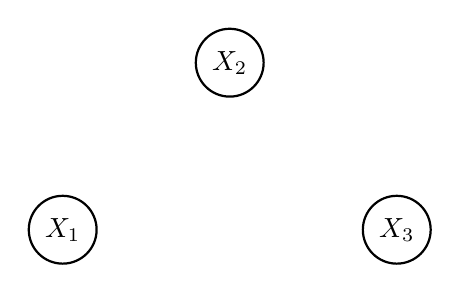
\begin{tikzpicture}[
            > = stealth, % arrow head style
            shorten > = 1pt, % don't touch arrow head to node
            auto,
            node distance = 3cm, % distance between nodes
            semithick % line style
        ]
	

        \tikzstyle{every state}=[
            draw = black,
            thick,
            fill = white,
            minimum size = 4mm
        ]
        
        \node[state] (x1) {$X_1$};
        \node[state] (x2) [above right of=x1]{$X_2$};
        \node[state] (x3) [below right of=x2] {$X_3$};

    \end{tikzpicture}
    
\bigskip
$1$ arc (Score 26.0)
\bigskip

    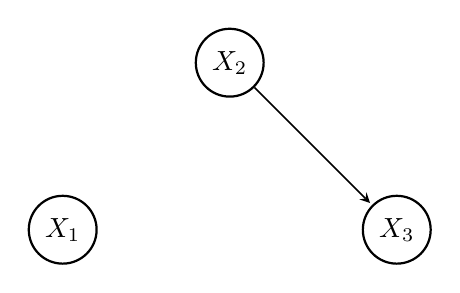
\begin{tikzpicture}[
            > = stealth, % arrow head style
            shorten > = 1pt, % don't touch arrow head to node
            auto,
            node distance = 3cm, % distance between nodes
            semithick % line style
        ]
	

        \tikzstyle{every state}=[
            draw = black,
            thick,
            fill = white,
            minimum size = 4mm
        ]
        
        \node[state] (x1) {$X_1$};
        \node[state] (x2) [above right of=x1]{$X_2$};
        \node[state] (x3) [below right of=x2] {$X_3$};

	\path[->] (x2) edge node {} (x3);
	
    \end{tikzpicture}
 
\bigskip
$2$ arcs (Score 19.0)
\bigskip

    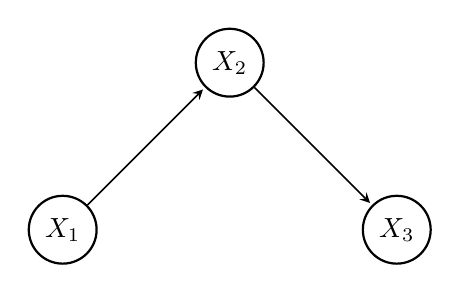
\begin{tikzpicture}[
            > = stealth, % arrow head style
            shorten > = 1pt, % don't touch arrow head to node
            auto,
            node distance = 3cm, % distance between nodes
            semithick % line style
        ]
	

        \tikzstyle{every state}=[
            draw = black,
            thick,
            fill = white,
            minimum size = 4mm
        ]
        
        \node[state] (x1) {$X_1$};
        \node[state] (x2) [above right of=x1]{$X_2$};
        \node[state] (x3) [below right of=x2] {$X_3$};

	\path[->] (x2) edge node {} (x3);
	\path[->] (x1) edge node {} (x2);
	
    \end{tikzpicture}

\bigskip
$3$ arcs (Score 15.0)
\bigskip

    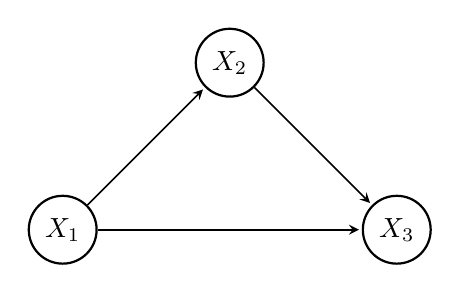
\begin{tikzpicture}[
            > = stealth, % arrow head style
            shorten > = 1pt, % don't touch arrow head to node
            auto,
            node distance = 3cm, % distance between nodes
            semithick % line style
        ]
	

        \tikzstyle{every state}=[
            draw = black,
            thick,
            fill = white,
            minimum size = 4mm
        ]
        
        \node[state] (x1) {$X_1$};
        \node[state] (x2) [above right of=x1]{$X_2$};
        \node[state] (x3) [below right of=x2] {$X_3$};

	\path[->] (x2) edge node {} (x3);
	\path[->] (x1) edge node {} (x3);
	\path[->] (x1) edge node {} (x2);
	
    \end{tikzpicture}

\subsection{DP for Constraining Number of Parentless Nodes}

Let $D(i, j)$ be the minimum value of $Sc(G, i)$ over all acceptable DAGs $G$ such that the number of nodes in $\{X_1,..., X_i\}$ with no parents is exactly $j$. 
We use the following recurrence. 

\bigskip{}
$D(0,0) = 0$

$D(0, z) = \infty$ for $z > 0$

\begin{equation}
    D(i, j) = \text{min}
    \begin{cases}
      D(i-1, j-1) + \sigma(X_i, \emptyset)\\
      \text{min} \{ D(i-1, j) + \sigma(X_i, p) : p \in \mathcal{P}_i \setminus \emptyset, \text{$ p$ respects }\theta \}
    \end{cases}
  \end{equation}
 
when $i > 0$. 

\bigskip{}
 To prove the recursive part of this formula, let $\hat{G}$ be any DAG over the ordering $\theta$ such that $Sc(\hat{G}, i) = D(i, j)$ and $\hat{G}$ has $j$ parentless nodes in the first $i$ nodes. If $X_i$ is parentless in $\hat{G}$, then $j-1$ of the first $i-1$ nodes in $\hat{G}$ are parentless, and moreover, $Sc(\hat{G}, i-1)$ must be minimal over all DAGs where $j-1$ of the first $i-1$ nodes are parentless (otherwise, we could again show $\hat{G}$ is not optimal). Hence, $Sc(\hat{G}, i) = D(i-1, j-1) + \sigma(X_i, \emptyset)$ for this case. 
 
 \bigskip{}
 The other case where $X_i$ is not parentless is very similar and yields $$Sc(\hat{G}, i) = \text{min} \{ D(i-1, j) + \sigma(X_i, p) : p \in \mathcal{P}_i \setminus \emptyset, \text{$ p$ respects }\theta \}$$
 
 Thus, the recursive formula provided considers all cases and therefore gives the optimal value over all acceptable DAGs. 


\subsection{DP for Both Constraints Simultaneously}

Let $D(i, j_1, j_2)$ be the minimum value of $Sc(G, i)$ over all acceptable DAGs $G$ such $A(G, i) = j_1$ and the number of nodes in $\{X_1,..., X_i\}$ with no parents is exactly
 $j_2$. 
 
 \bigskip{}
$D(0, 0, 0) = 0$

$D(0, z_1, z_2) = \infty$ for $z_1 > 0$ or $z_2 > 0$. 

\begin{equation}
    D(i, j_1, j_2) = \text{min}
    \begin{cases}
      D(i-1, j_1, j_2-1) + \sigma(X_i, \emptyset)\\
      \text{min} \{ D(i-1, j_1 - |p|, j_2) + \sigma(X_i, p) : p \in \mathcal{P}_i \setminus \emptyset, \text{$ p$ respects }\theta \}
    \end{cases}
  \end{equation}

\bigskip{}
The proof of correctness is similar to those for the above cases. In the computation for $D(i, j_1, j_2)$ we consider all choices of parent sets for $X_i$. Note the similarity of this problem to the \textit{Knapsack Problem}, where each item has two weight properties (say, ``weight" and ``size") and we wish to maximize/minimize the value of items selected given limits on both weight properties. Number of arcs can be thought of as ``weight" and number of parentless nodes can be thought of as ``size". A parent set $p$ has ``weight" $|p|$ and ``size" $1$ if $p$ is empty, $0$ otherwise. 


\end{document}
